\begin{titlepage}
{\sffamily
\maketitle
\begin{center}
    \vfill
    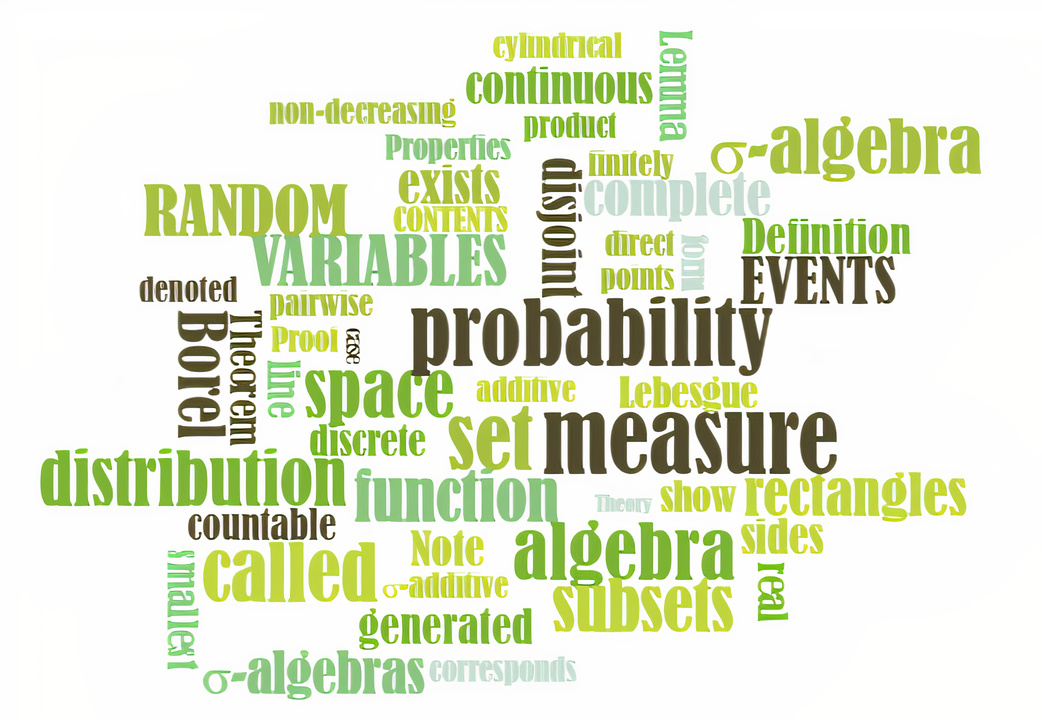
\includegraphics[scale = 1.7]{mypic.jpg}
    
    \vspace{4cm}
    \Large
    Department of Mathematics\\
    \textit{Imperial College London}\\
\end{center}}
\end{titlepage}
\newpage

We have written this set of unofficial notes to facilitate your understanding of important concepts in Probability Theory. Although most parts of the notes are based the lecture videos and in-person lectures given by Dr. Igor Krasovsky in Spring 2022, we have included additional materials drawn from various references. In particular: 

\begin{unexaminable}
\begin{itemize}
    \item Any unexaminable materials are highlighted using gray colorboxes.
\end{itemize}
\end{unexaminable}
\begin{itemize}
    \item Any unfinished/planned materials are written in \red{red}.
\end{itemize}

\textbf{Disclaimer.} These notes have not been checked by Dr. Krasovsky and should not be regarded as a replacement of the official notes and lectures for the course. In particular, all the errors are made by us, and we don't take any responsibility for their consequences; use at your own risk (and please do attend lectures -- they are fun). \\

Please email us at (insert email) with any comments or corrections.\\

Ivan Kirev and Samuel Lam \\
September 2022\\

\begin{center}
\framebox{{\sffamily Version: 0.1.2, Date: \today}}
\end{center}

\newpage 

{\pagestyle{empty}
\tableofcontents}
\newpage